\chapter{告発する約束・評判ゲーム}
本章では、\ref{hypothesis}節で定義した補題2を検証する。

\section{補題2}
\secondLemma
% 成員の行動を観察できない外部の強制執行力が存在すると仮定した上で、集団を構成する成員達の性質によっては、
% 成員達に合意された約束を履行させるインセンティブ設計が可能である。

\section{提案手法}
不正行為にあった場合に必ず「失敗」を報告する行動を「告発」と呼び、
「告発」するプレイヤーのみが参加する「約束・評判ゲーム」を「告発する約束・評判ゲーム」としてモデリングする。
この「告発する約束・評判ゲーム」において、不正が防止される条件を導き出す。
そして、その条件を満たす「評判システム」を通常の「約束・評判ゲーム」に適用し、
様々な戦略をとるエージェントを用いてマルチエージェントシミュレーションを行ことで、
集団を構成する成員達の性質によっては、成員達に合意された約束を履行させるインセンティブ設計が可能であることを示す。

\section{告発}
\ref{verification1}節の検証では、
「評判システム」から$reporter$が戦略$s_{r1}$と$s_{r4}$をとる確率$p_{r1}$と$p_{r4}$を推定できないため、
不正を防止する$(r_{ps}, r_{pf}, r_{ps}, r_{pf})$の組を決定することができなかった。

\section{告発約束・評判ゲーム}
「倫理」に従うプレイヤーのみで行われる「約束・評判ゲーム」を「告発する約束・評判ゲーム」とする。
このゲームにおいては、step1で$promisor$が約束を履行しなかった場合、$reporter$は必ず「失敗」を報告するため、
ゲームの木は図\ref{ethical-gametree}のようになる。
また、\ref{playersStrategy}節で示した$reporter$の戦略のうち$s_{r2}$と$s_{r4}$がとられないため、
非協力戦略型ゲームとして表したときの利得は表\ref{ethical-gametable}のようになる。

\begin{figure*}
  \centering
  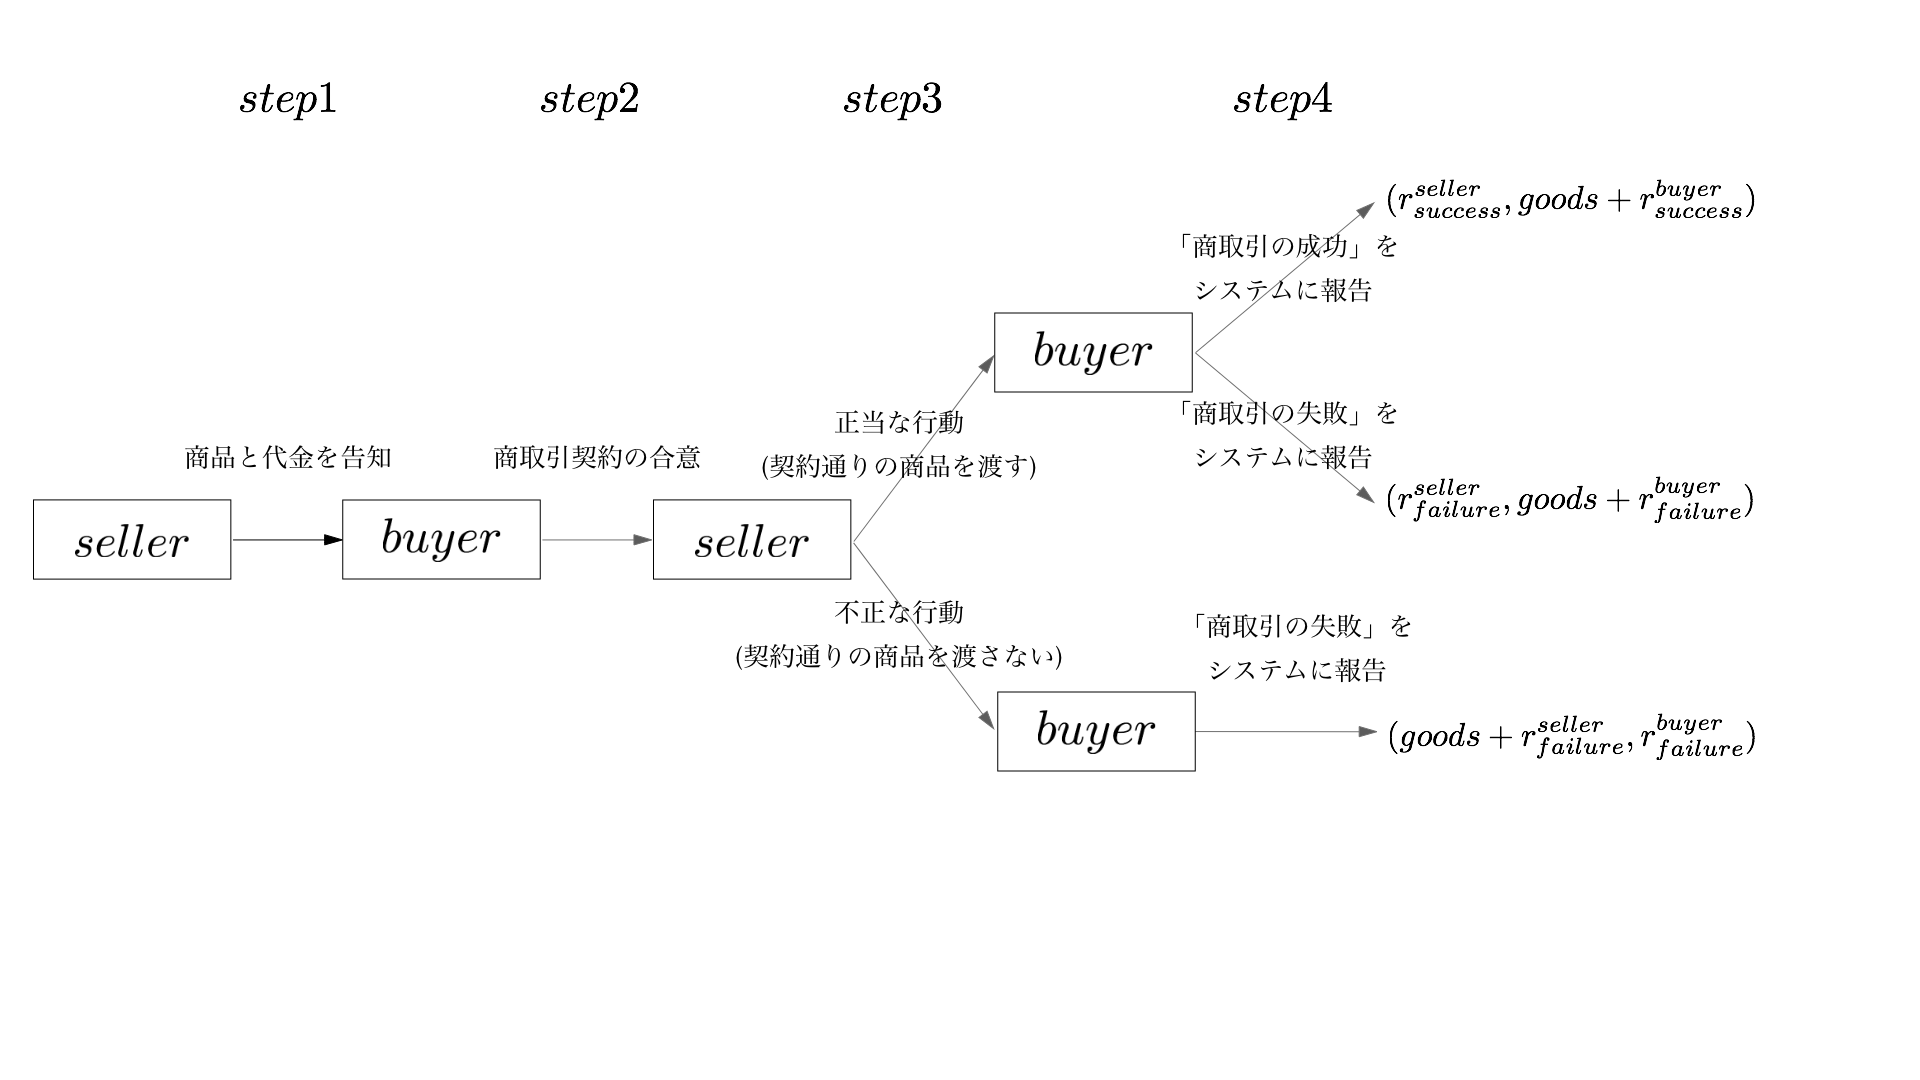
\includegraphics[width=1\linewidth]{./06_ethical-prgame/ethical-gametree.png}
  \caption{「告発する約束・評判ゲーム」のゲーム木}
  \label{ethical-gametree}
\end{figure*}

% Success Reported on True Success
\newcommand{\SROS}{ $(c_{p1} + r_{ps},$ \\$c_{r1} + r_{rs})$ }
\newcommand{\FROF}{ $(c_{p2} + r_{ps},$ \\$c_{r2} + r_{rs})$ }
\newcommand{\FROS}{ $(c_{p1} + r_{pf},$ \\$c_{r1} + r_{rf})$ }
\newcommand{\SROF}{ $(c_{p2} + r_{pf},$ \\$c_{r2} + r_{rf})$ }
\newcommand{\tabularc}[1]{\begin{tabular}{c} #1 \end{tabular}}

\begin{table*}[h]
  \begin{tabular}{|l|l|l|l|l|l|}
  \hline
  \multicolumn{2}{|l|}{\multirow{2}{*}{}} & \multicolumn{4}{l|}{$Reporter$} \\ \cline{3-6}
  \multicolumn{2}{|l|}{}                  &$s_{r1}$&$s_{r2}$&$s_{r3}$&$s_{r4}$\\ \hline
  \multirow{2}{*}{$Promisor$}
  &$s_{p1}$&\tabularc{\SROS}&\tabularc{\SROS}&\tabularc{\FROS}&\tabularc{\FROS}\\ \cline{2-6}
  &$s_{p2}$&\tabularc{\SROF}&\tabularc{\FROF}&\tabularc{\SROF}&\tabularc{\FROF}\\ \hline
  \end{tabular}
  \caption{「約束・評判ゲーム」の利得票表}
  \label{prgametable}
\end{table*}

\section{不正が防止される条件}
表\ref{prgametable}より,「告発する約束・評判ゲーム」において、約束が履行されるためには、
$promisor$と$reporter$のとる戦略組が$ (s_{p1}, s_{r1})$になる必要がある.
各プレイヤーが戦略$s$をとったときの利得を$R$とし、その期待値を$E(R|s)$とする。
全てのプレイヤーが完全に合理的な場合、戦略組$(s_{p1}, s_{r1})$に帰着させるためには,

\begin{description}
  \centering
  \item[条件③] $E(r|s_{p1}) > E(r|s_{p2})$かつ$E(r|s_{r1}) > E(r|s_{r3})$
\end{description}

を満たす$(r_{ps}, r_{pf}, r_{rs}, r_{rf})$の組を「評判システム」から決定できる必要がある.

\subsection{各戦略の期待利得}
$promisor$と$reporter$の各戦略の期待利得は次のように表せる.

\begin{eqnarray}
  E(R|s_{p1}) &=& p_{r1} (r_{ps} + \epsilon^{promiser}) + p_{r3} (r_{pf} + \lambda^{promiser}) \\
  E(R|s_{p2}) &=& p_{r1} (goods + r_{pf} + \lambda^{promiser}) + p_{r3} (goods + r_{pf} + \lambda^{promiser}) \\
              &=& goods + r_{pf} + \lambda^{promiser} \because p_{r1} + p_{r3} = 1 \\
  E(R|s_{r1}) &=& p_{p1} (goods + r_{rs} + \epsilon^{reporter}) + p_{p2} (r_{rf} + \lambda^{reporter}) \\
  E(R|s_{r3}) &=& p_{p1}(goods+r_{rf} + \lambda^{reporter}) + p_{p2} (r_{rf} + \lambda^{reporter}) \\
              &=& p_{p1} goods + r_{rf} + \lambda^{reporter} \because p_{p1} + p_{p2} = 1
\end{eqnarray}


\subsection{$promiser$が$s_{p1}$をとる条件}

$ E(R|s_{p1}) > E(R|s_{p2}) $を満たすためには、
\begin{eqnarray*}
  &&E(R|s_{p1}) > E(R|s_{p2}) \\
  &\therefore& p_{r1} (r_{ps} + \epsilon) + p_{r2} (r_{pf} + \lambda) > goods + r_{pf} + \lambda \\
  &\therefore& p_{r1}(r_{ps} + \epsilon) - p_{r1}(r_{pf} + \lambda) > goods \\
  &\therefore& p_{r1}(r_{ps} - r_{pf} + \epsilon - \lambda) > goods
\end{eqnarray*}

仮定より,$ \epsilon > \lambda $のため,

\begin{equation}
  p_{r1} (r_{ps} - r_{pf}) \geq goods
\end{equation}

を満たせばよい.

\subsection{$reporter$が$s_{r1}$をとる条件}

$ E(R|s_{r1}) > E(R|s_{r3}) $を満たすためには、
\begin{eqnarray*}
  &&E(R|s_{r1}) > E(R|s_{r3}) \\
  &\therefore& p_{p1} (goods + r_{rs}) + p_{p2} r_{rf} > p_{p1}(goods+r_{rf}) + p_{p2} r_{rf} \\
  &\therefore& p_{p1}(r_{rs} - r_{rf}) > 0 \\
\end{eqnarray*}

を満たせばよい。


\subsection{戦略組($s_{p1}$, $s_{r1}$)に帰結する条件}

$ 0<p_{r1} $かつ $ 0 < p_{p1}$を仮定した上で,\\

\begin{equation}
  r_{ps} - r_{pf} \geq \frac{goods}{p_{r1}}
\end{equation}

かつ

\begin{equation}
  r_{rs} - r_{rf} > 0
\end{equation}

を満たせば,「倫理ある商取引ゲーム」で不正を防止することができる.

\subsection{誠実な戦略をとった割合と成功が報告される割合の関係}
% メモ:要修正
ここで、「告発する約束・評判ゲーム」において,全ての成員は「告発」するため、
真の成功率は「評判システム」に「成功」が報告された割合以上となる。

つまり、任意の成員$i$と$j$が過去に「約束・評判ゲーム」を行った際に、
$s_{p1}$をとってきた割合$HonestStrategyRate(p, q)$と、
成功が報告された割合$ReportedSuccessRate(p, q)$について、次の関係がいえる。

\begin{equation}
  HonestStrategyRate(i, j) \geq ReportedSuccessRate(i, j)
\end{equation}


\subsection{信頼度 $ P_i $}

ここで、成員$i$が$s_{p1}$をとる主観確率$ p_{p1} $と$P_i$とし,
$ P_i $を$HonestyStrategyRate(i, j)$と
$\sum^{\{1, 2, ..., n\}}_{k}w_k = 1$を満たす任意の重み$ w_k $ ($k \in \{1, 2, ..., n\}$)を用いて次のように定義する. \\

\begin{equation}
  p_i \equiv \sum^{\{1,2,..., n\}}_{j} w_{j} \cdot HonestyStrategyRate(i, j)
\end{equation}


\subsection{最低信頼度 $ T_i $}
「評判システム」から$HonestyStrategyRate(i, j)$は未知のため,信頼度$ p_{p1} $を求めることができない.
そこで$ HonestyStrategyRate $の代わりに$ ReportedSuccessRate $を用い、
信頼度$ p^{player} $を計算するのと同じ重み$ w^{player} $の荷重総和をとったものを、
最低信頼度$ T_i $と定義する. \\

\begin{equation}
  T_i \equiv \sum^{\{1,2,..., n\}}_{j} w_j \cdot HonestyStrategyRate(i, j)
\end{equation}

ここで$ HonestyStrategyRate \geq ReportedSuccessRate $であるため,$ P_i \geq T_i $がいえる.


\subsection{最低信頼度を用いた条件}

ゆえに,

\begin{equation}
  r_{ps} - r_{pf}  \geq \frac{goods}{T^{reporter}} \geq \frac{goods}{p_{r1}}
\end{equation}

となる.

つまり、$ 0<p_{r1} $かつ $ 0 < p_{p1}$を仮定した上で,\\

\begin{equation}
  r_{ps} - r_{pf} \geq \frac{goods}{T_i} かつ r_{rs} - r_{rf} > 0
\end{equation}

を満たす$ (r_{ps}, r_{pf}, r_{rs}, r_{rf}) $の組を「評判システム」から決定できれば、
「告発する信用・評判ゲーム」において不正を防止することができる。

\section{評判システムの詳細}
本節ではシミュレーションに用いる「評判システム」の仕様の詳細を紹介する。
完全な実装については、GitHubのソースコードを参照。

\subsection{約束の価値$C$}
\begin{eqnarray}
  C &\equiv& 1 \\
    &=& c_{p2} - c_{p1} \\
    &=& c_{r1} - c_{r2}
\end{eqnarray}

\subsection{ReputationWeight}
最低信頼度$ T_i $を求めるため、$ReportedSuccessRate(i, j)$の荷重総和に用いる重み$ w_k $を定義する.
この重み$w_k$は、任意の成員$i$が戦略$s_{p1}$をとる確率$p_{p1}$を推定する際に、
成員$i$と他の成員$j$における$ReportedSuccessRate(i, j)$をどの程度信頼するかを表している。
本実験では、成員$j$の「評判スコア」が全体に占める割合をReputationWeight$w_j$と定義する。
任意の成員$k$の「評判スコア」を$b_k$としたとき、$w_k$は次のように表せる。($n$は成員の人数)

\begin{equation*}
  w_k \equiv \frac{b_k}{\sum^{\{1,2,...,n\}}_{k}b_k}
\end{equation*}

\subsection{「成功」が報告された場合の「評判スコア」の変化}
$ reporter $が「成功」を報告した場合、
$ reporter $は約束の価値$C$だけ減り、$ promisor $は$C$だけ増加するものとする。

\begin{gather}
  r_{ps} = C \\
  r_{rs} = -C \\
  r_{ps} + r_{rs} = 0
\end{gather}


\subsection{EscrowCost}
「失敗」が報告されたとき、$promisor$と$reporter$が失う「評判スコア」の合計を$EscrowCost$とする。
約束の価値$C$にエスクロー係数$E$を掛けたものとする.

\begin{eqnarray}
  EscrowCost  &\equiv& (r_{rs} - r_{rf}) + (r_{ps} - r_{pf}) \\
              &=& E \cdot C \label{escrowCost}
\end{eqnarray}

\subsection{EscrowCostの負担比率}
成員$i$を$promiser$、$j$を$reporter$とする。
「約束・評判ゲーム」を行うとき、$EscrowCost$の負担比率を両者の最低信頼度$T_i$を用いる.\\

\begin{equation}
  (r_{ps} - r_{pf}):(r_{rs} - r_{rf}) = T_j:T_i
\end{equation}

\subsection{EscrowCostの分配}
「失敗」が報告されたときに$EscrowCost$が消失すると、
「評判スコア」の総量が下がり、約束の価値$C$

総量を一定に保つために、$promisor$と$reporter$以外の全てのプレイヤーに、
$ReputationWeight$に応じて$EscrowCost$を分配する。
$promisor$と$reporter$を含まないのは、分配によるインセンティブ設計への影響をなくすためである。

\subsection{不正が防止される条件を満たす定義}
成員$j$を$promiser$、$k$を$reporter$とする。
このとき、\eqref{condition6-1}と\eqref{condition6-2}を満たす$r_{ps} - r_{pf}$と$r_{rs} - r_{rf}$を下記のように定義する。

\begin{eqnarray}
  r_{ps} - r_{pf} &\equiv& \frac{C}{T_i} \label{condition6-3} \\
                  &\geq& \frac{c_{p2} - c_{p1}}{T_i} \nonumber \\
  r_{rs} - r_{rf} &\equiv& \frac{C}{T_j} \label{condition6-4} \\
                  &\geq& 0 \nonumber
\end{eqnarray}

\subsection{残高の変化量の組$ (r_{ps}, r_{pf}, r_{rs}, r_{rf}) $}
上記の定義からエスクロー係数$E$と残高の変化量の組$ (r_{ps}, r_{pf}, r_{rs}, r_{rf}) $は次のように求まる. \\
成員$i$を$promisor$、$j$を$reporter$とする。

\begin{eqnarray}
  E &=& - \frac{T_i + T_j}{T_i T_j} \\
  r_{ps} &=& 1 \\
  r_{pf} &=& 1 - \frac{1}{T_j} \\
  r_{rs} &=& -1 \\
  r_{rf} &=& -1 - \frac{1}{T_i}
\end{eqnarray}


\section{実験方法}
先の不正が防止される条件を満たすインセンティブ設計を行う「評判システム」と
次の8タイプのエージェントから重複問わずランダムに選んだ8体のエージェントを用意し試行を実施する。
これをタイプAのエージェントが0〜7体を占める場合について、それぞれ8000回づつ繰り返し、
エージェントの構成とstep13で求まる「報告された成功率」と「真の成功率」を記録する。

\subsection{エージェントの種類}
下記のA~Hの8タイプのエージェントを用意する。
\begin{description}
  \item [A] 約束を履行し、$promisor$が約束を履行したとき「成功」、反故にしたとき「失敗」を報告する。
  \item [B] 約束を履行し、$promisor$が約束を履行したとき「成功」、反故にしたとき「成功」を報告する。
  \item [C] 約束を履行し、$promisor$が約束を履行したとき「失敗」、反故にしたとき「成功」を報告する。
  \item [D] 約束を履行し、$promisor$が約束を履行したとき「失敗」、反故にしたとき「失敗」を報告する。
  \item [E] 約束を反故にし、$promisor$が約束を履行したとき「成功」、反故にしたとき「失敗」を報告する。
  \item [F] 約束を反故にし、$promisor$が約束を履行したとき「成功」、反故にしたとき「成功」を報告する。
  \item [G] 約束を反故にし、$promisor$が約束を履行したとき「失敗」、反故にしたとき「成功」を報告する。
  \item [H] 約束を反故にし、$promisor$が約束を履行したとき「失敗」、反故にしたとき「失敗」を報告する。
\end{description}

\subsection{試行}
\begin{description}
  \item[step 1] 時刻tを0とする。
  \item[step 2] 「評判システム」の各エージェントの初期の「評判スコア」を8とする。
  \item[step 3] 全てのエージェントが$promisor$と$reporter$として1度ずつ総当りする順序を決定する。(順序の長さは56となる)
  \item[step 4] 時刻tを1進める。
  \item[step 5] step 3で決定した順序を周期として、$promisor$と$reporter$を決定する。
  \item[step 6] 「評判システム」は「成功」と「失敗」が報告された場合の$promisor$と$reporter$の「評判スコア」を計算する。
  \item[step 7] $promisor$は自身の戦略に基づいて約束を履行するか反故にする。
  \item[step 8] $reporter$は自身の戦略とstep 6の$promisor$の行動に基づいて結果を決定する。
  \item[step 9] $reporter$は決定した結果を「評判システム」に報告する。 
  \item[step 10] 「評判システム」はstep6で計算した「評判スコア」がいずれの場合にも0未満にならない場合、 reporterから報告された結果を記録する。
  \item[step 11] step6で計算した「評判スコア」がいずれの場合にも0未満にならない場合、真の結果を記録する。
  \item[step 12] 時刻tが1120未満なら、step4に戻る。
  \item[step 13] 過去56回の約束・評判ゲームにおいて、step10と11で記録された結果を集計し、それぞれ「報告された成功率」と「真の成功率」を求める。
\end{description}

\section{評価}
先の実験の結果、「報告された成功率」と「真の成功率」の両方が100\%になった場合を「不正防止の成功」とし、
誠実なエージェント(タイプA)の数と「不正防止の成功」に至った割合をプロットしたものが、図\ref{ethical-game-001}である。
(エージェント数8の場合は、エージェントの組み合わせが1通りしか存在しないため、個別に試行を行い結果を集計している。)
誠実なエージェントの数が0体の場合であっても不正が防止される構成が存在し、
6体以上の場合はサンプリングした全ての構成で不正の防止が成功していた。

\begin{figure}[h]
  \begin{tabular}{cc}
    \begin{minipage}[t]{1\hsize}
      \centering
      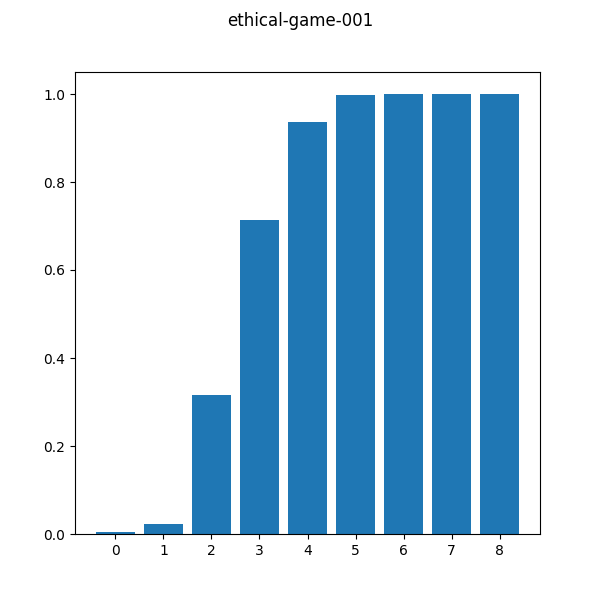
\includegraphics[keepaspectratio, width=1\linewidth]{./06_ethical-commerce-game/ethical-game-001.png}
      \caption{誠実なエージェントの数と「不正防止の成功」に至った割合}
      \label{ethical-game-001}
    \end{minipage}
  \end{tabular}
\end{figure}

\section{結論}
実験とその評価から、「告発」という限定合理性を仮定した上でインセンティブ設計を行うことで、
プレイヤーの構成によっては「約束・評判ゲーム」において不正を防止することが可能であることがわかる。
プレイヤーの構成と不正防止の成功成功の関係性については、先の実験の図\ref{ethical-game-001}のとおりである。
